\section{Separate Chaining}%
\label{sec:separate_chaining}

\begin{frame}
	\frametitle{Separate Chaining}
	\begin{center}
		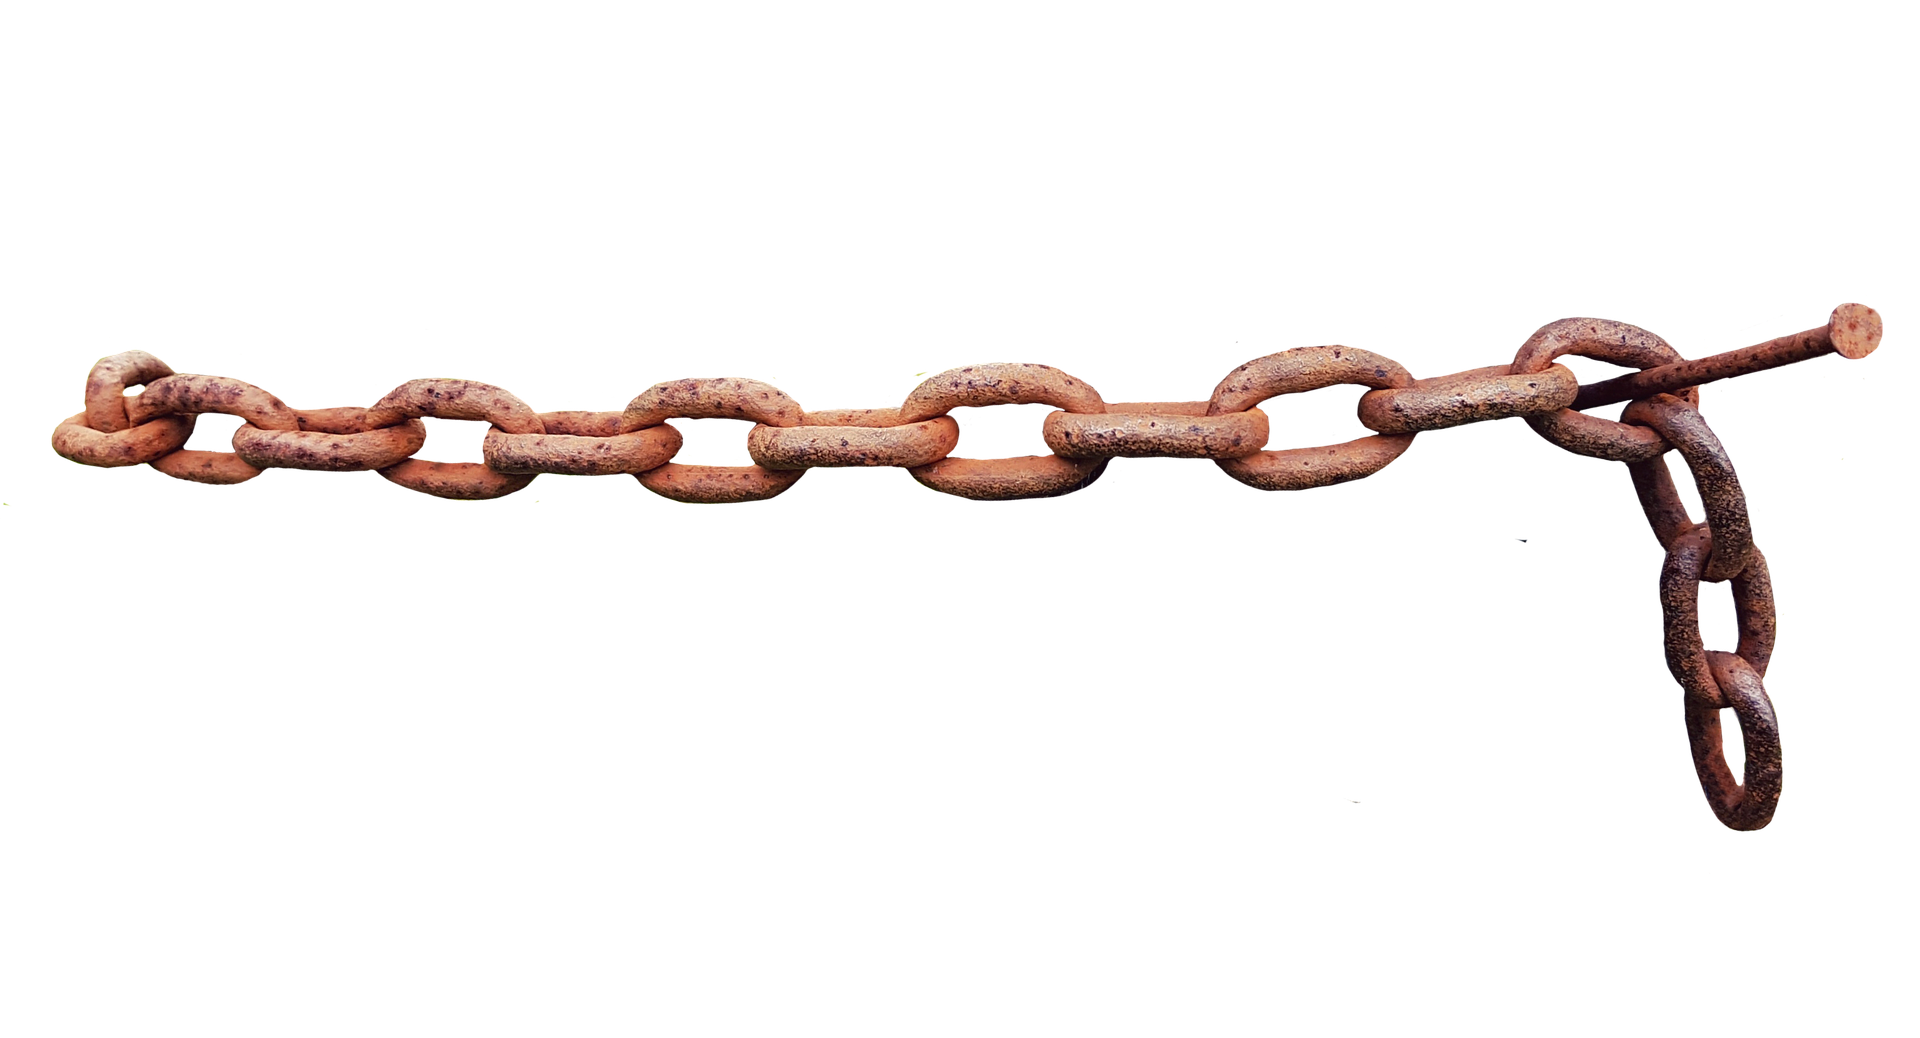
\includegraphics[width=0.8\textwidth]{figures/chains.png}\\
		\hspace*{15pt}\hbox{\scriptsize Image By:\thinspace{\itshape Prettysleepy2}}
	\end{center}
\end{frame}

\begin{frame}
	\frametitle{Separate chaining}
		\begin{block}{Separate chaining}
			Every bucket is a linked list. It can just hold more items as needed.\\
			Easy to implement, but overhead in terms of space for the linked lists.
		\end{block}	
		\pause
		\begin{questionblock}{Quick practice}
		  Take hash function $f(k) = 2k + 3$ and a map of \textit{fixed} size $10$. What does a map look like that has the
			keys: $1,2,7,12,13,19,22,27$?
		\end{questionblock}
		\pause
		\begin{answerblock}{Lets draw it}
			We have a smart board available.
		\end{answerblock}
\end{frame}

\begin{frame}
	\frametitle{In Python}
	\lstinputlisting{code/sepchain.py}
\end{frame}
